% !TeX root = ../main.tex

%\section{Killer Whale Case Study}

\subsection{Data Collection and Preprocessing}

To demonstrate this methodology as applied to real-world data, the CarHHMM was used to analyze dive data from a killer whale off the coast of British Columbia, Canada. The data was collected on September 2, 2019 from 12:49 pm to 6:06 pm and consists of depth and acceleration in three orthogonal directions. Observations were collected at a rate of 50 hertz. Tagging the killer whale caused anomalous behavior before 1:20 pm and after 6:00 pm, so observations in this time range were ignored. In addition, the tagging technology dropped data between 2:25pm and 2:37pm as well as between 4:07 and 5:07 pm, so any partially observed data within this time range were ignored as well. A killer whale ``dive" is considered to be any continuous chunk of data that occurs below 0.5 meters in depth and lasts for at least 10 seconds. This process resulted in a total of 267 dives. Accelerometer and depth data were smoothed by taking a moving average with a window of 1/10th of a second. Data preprocessing was done in part with the \textit{divebomb} package in Python \cite{Nunes:2018}.

\subsection{Model Selection}

The collection of all dive durations were set to be the coarse-scale observations $Y$, and the acceleration data was used to determine the fine-scale observations $Y^*$. Figure (\ref{fig:raw_data_one_dive}) shows both the depth profile and the raw accelerometer data for one specific dive. The acceleration exhibits sinusoidal behavior at several points in time which cannot be modeled using HMMs without signal processing of the raw acceleration data. Therefore, the STFT was used to process the raw acceleration data and calculate both $Y{*(1)}$ and $Y^{*(2)}$. We set $\tilde{f} = 5$ hertz and $h = 2$ seconds, which reduced the dimension of each window from $50 s^{-1} * 2 s = 100$ to 2.

In order to find if the CarHHMM was appropriate for this data, a lag plot was made for both $Y^{*(1)}_{t,s^*}$ and $Y^{*(2)}_{t,s^*}$. The results of doing so are shown in figure (\ref{fig:lag}). Unfortunately, the number of behavioral states is not clear from the lag plot, but it is clear that $Y^{*(1)}_{t,s^*}$ exhibits a large degree of auto-correlation. While $Y^{*(2)}_{t,s^*}$ also exhibits some auto-correlation, the relationship is less strong, so auto-correlation was not incorporated in the emission distribution of $Y^{*(2)}_{t,s^*}$. 

\begin{figure}[h!]
	\centering
	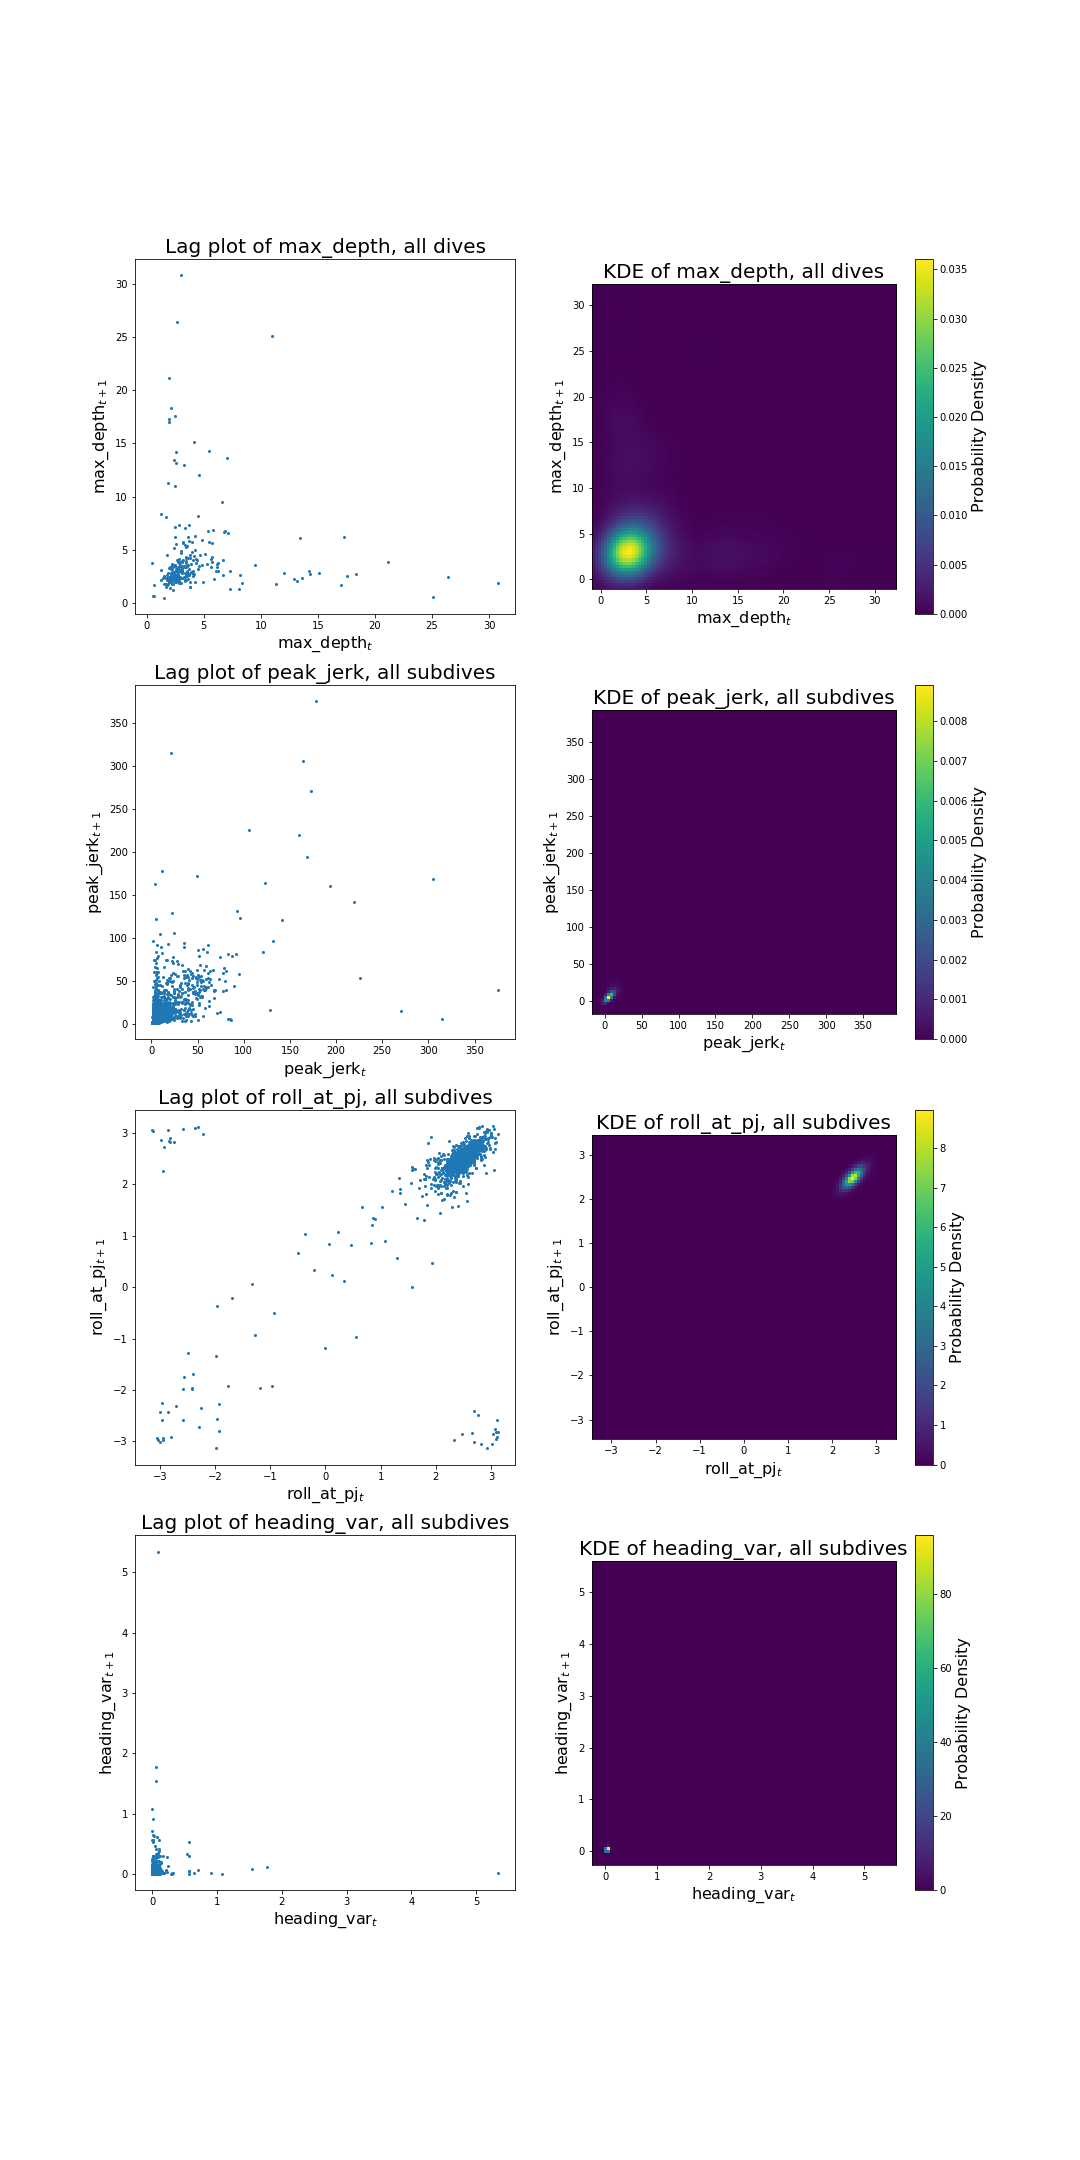
\includegraphics[height=5in]{../Plots/lagplot.png}
	\caption{Lag plot of vertical velocity and $\tilde a$ (left) and a the associated normal kernel density estimates (right)}
	\label{fig:lag}
\end{figure}

Since information criteria tend to overestimate the number of states in biological processes \cite{Pohle:2017}, we instead selected $N = 2$ dive types and $N^* = 3$ sub-dive behaviours heuristically and admittedly somewhat arbitrarily.

\subsection{Results}

The parameters of the estimated emission distributions for each behavioral state are shown in table (\ref{table:emis_dist}). Each distribution is also plotted in figure (\ref{fig:emis_dist}). Note that the auto-correlation within the velocity sequence is not captured in figure (\ref{fig:emis_dist}), so it is important to refer to the estimated auto-correlation parameter $\hat \phi$ from table (\ref{table:emis_dist}) when considering the emission distributions shown in figure (\ref{fig:emis_dist}).
%
\begin{figure}[h!]
	\centering
	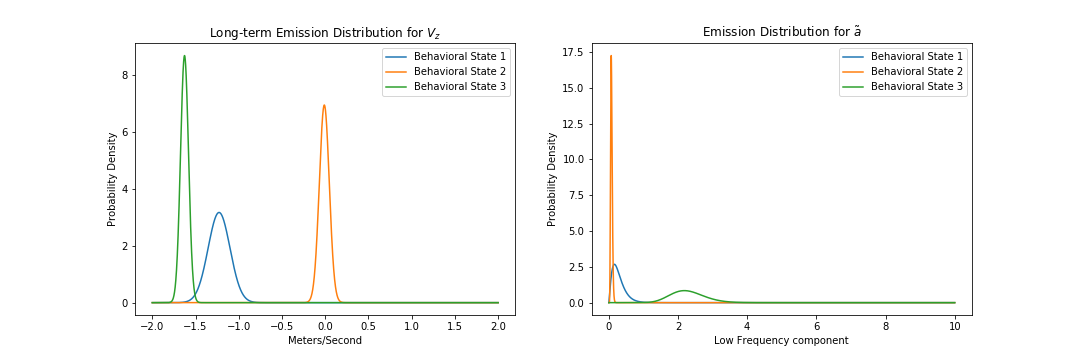
\includegraphics[height=2in]{../Plots/emis_dist.png}
	\caption{Estimated probability distributions for the long-term vertical velocity and $\tilde a$ in each behavioral state. Note that the distribution over vertical velocity does not take autocorrelation into account.}
	\label{fig:emis_dist}
\end{figure}
%
\begin{table}[h!]
	\centering
	\begin{tabular}{l|lll}
		& State 1 & State 2 & State 3 \\ \hline
		$\hat \mu_{RL}$        & 0.66    & 0.68    & 0.22    \\
		$\hat \sigma^2$        & 0.095   & 0.070   & 1.30    \\
		$\hat \phi$            & 0.88    & 0.99    & 0.03    \\ \hline
		$\hat \tilde \mu$      & 0.69    & 0.15    & 3.70    \\
		$\hat \tilde{\sigma^2}$ & 0.41    & 0.067   & 3.16   
	\end{tabular}
	\caption{Table of estimated parameters for probability distributions over $v$ and $\tilde a$ for each behavioral state}
	\label{table:emis_dist}
\end{table}
%
The estimated probability transition matrix and associated stationary distribution is shown below:

$$\hat \Gamma = \begin{pmatrix} 
0.7983 & 0.1618 & 0.0398 \\
0.0120 & 0.8796 & 0.0003 \\
0.2425 & 0.0049 & 0.7526
\end{pmatrix} \qquad \hat \delta = \begin{pmatrix} 0.4141 & 0.5020 & 0.0839 \end{pmatrix}$$

Finally, the Viterbi-decoded dive behavior within a randomly selected dive (deeper than 20 meters) is shown in figure (\ref{fig:viterbi}).

\newpage

\begin{figure}[h!]
	\centering
	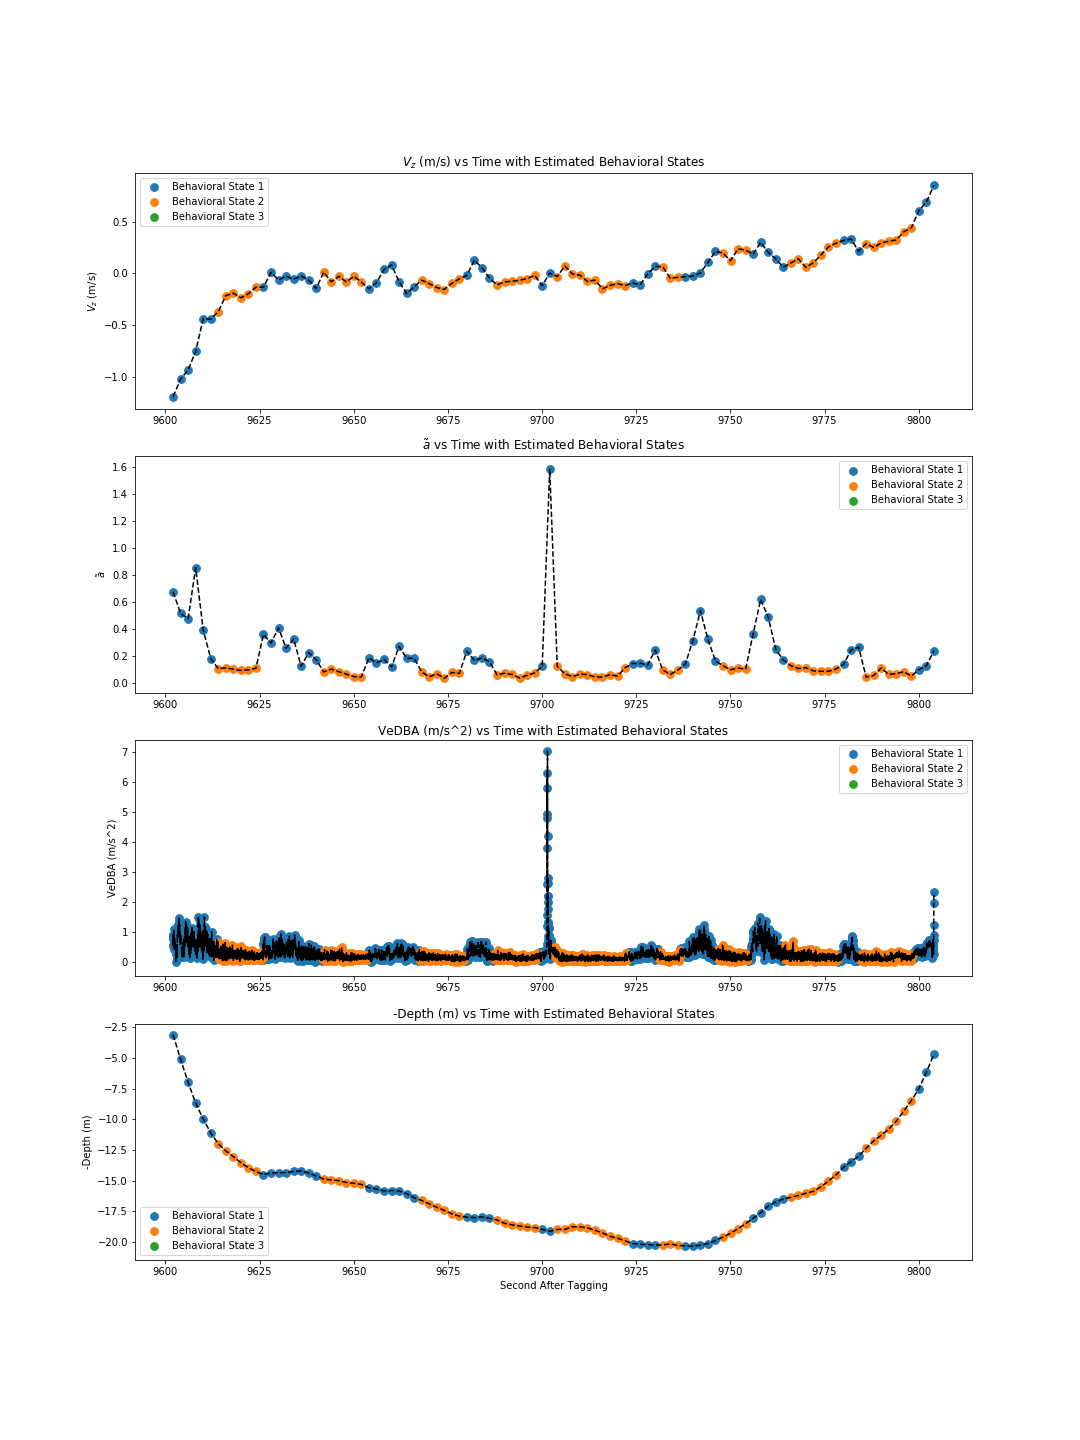
\includegraphics[height=8in]{../Plots/viterbi.png}
	\caption{Features of a particular killer whale dive and Viterbi-decoded estimates for the intra-dive behavioral states.}
	\label{fig:viterbi}
\end{figure}

\newpage

While the ecological meaning of these behavioral states is tenuous, we hypothesize the following interpretations. Roughly speaking, behavioral state 1 corresponds to mildly active swimming. The mean of $\tilde a$ in this state is larger than behavioral state 2, indicating more activity by the whale, but the autocorrleation term $\hat \phi$ is still very high, indicating that velocities don't change very much every two seconds. Behavioral state 2 corresponds to gliding or turning, where no active swimming is taking place. It is characterized by a low mean $\tilde a$ value and a very high autocorrelation term $\hat \phi$, both of which indicate little activity. Finally, behavioral state 3 represents sudden jerking or more vigorous and active swimming than behavioral state 1. This behavior is so rigorous that $\hat \phi$ drops almost to zero and $\hat \sigma^2$ subsequently rises significantly. In behavioral state 3, the velocity readings of the killer whale are essentially uncorrelated when recorded every two seconds.

\subsection{Future Work}

This analysis is largely exploratory with a purely heuristic approach to decide the number of behavioral states. Future work should repeat the analysis using several different values for the number of behavioral states. It is also important to validate these results by plotting psuedoresiduals and performing goodness-of-fit tests on the emission distributions.

Parameter estimation via likelihood maximization can be slow, especially with an observation rate of 50 hertz. If dives are modeled as uncorrelated batches of data, then using stochastic gradient ascent to maximize the likelihood may considerably speed up parameter estimation.

Finally, this work was run exclusively on dives deeper than 20 meters so that within-dive behaviors would be similar between dives. Future analysis could find a way to include a more heterogeneous set of dives using a framework such as the hierarchical hidden Markov model (HHMM) introduced by Leos-Barajas et al \cite{Barajas:2017}.

\subsection{Model evaluation}

